%\chapter{案例研究 2：用于大语言模型推理与反思的 BALROG}\label{chap:balrog}
\chapter[案例研究 2：推理与反思]{案例研究 2：用于大语言模型推理与反思的 BALROG}\label{chap:balrog}

\begin{learningbox}
在本案例研究中，你将获得构建面向推理领域的自反思智能体的动手经验。
具体而言，你将能够：
\begin{itemize}[leftmargin=*, nosep]
    \item 在谜题与游戏基准上运行一个多步{\em 推理智能体}。
    \item 用自己的想法改造推理智能体。
    \item 实现你自己的{\em 自反思}智能体。
    \item 批判性地反思学习智能体在谜题与游戏领域中的{\em 性能与稳定性}。
\end{itemize}
\end{learningbox}

\section{BALROG 概览}
%We will discuss a practical 
本案例中，我们将使用一个执行自反思的智能体式大语言模型。我们采用一套流行的推理任务基准，称为 BALROG。\footnote{Balrog（炎魔）是 J.R.R. 托尔金奇幻作品中登场的中土神话恶魔。一只炎魔足以与最强大的巫师灰袍甘道夫匹敌。} BALROG 是 {\em B}enchmarking {\em A}gentic {\em L}LM and VLM {\em R}easoning {\em O}n {\em G}ames（在游戏上评测智能体式大语言模型与视觉语言模型的推理能力）的首字母缩写。BALROG 基准由易、难游戏混合构成，其中一些游戏连大语言模型都难以玩好，正如 BALROG 论文在其自身的基准研究中所展示的 \citep{paglieri2024balrog}。

最初，BALROG 游戏是用原生大语言模型来评测的。不过，其代码相当开放，便于你编写自己的智能体方法，看看能否做得更好。
%The BALROG suite is designed in a way to invite others to use it. 
这套软件的设计目的，就是让你为上下文（强化）学习编写自己的智能体代码。



%In this chapter we will use the BALROG  benchmarks to experiment with the reasoning and self reflection  approaches that we discussed in the previous  chapters.

\begin{comment}
    

\section{Learning Goals}
The  goal of this chapter is to better understand the  capabilities reasoning models and self reflection mechanisms, and their weaknesses. This experience will help you understand the challenges faced when designing reasoning and self-reflection agents for your applications.


After completing this case, you should be able to:
\begin{enumerate}
    \item Implement an agentic LLM system with explicit planner and executor roles
    \item Run the agent on challenging plannign-type problems
    \item Evaluate, debug and analyze experimental results
    \item Critically reflect on the capabilities of reasoning agents on challenging puzzle and game benchmarks
\end{enumerate}
\end{comment}



BALROG 的主网站是 \url{https://balrogai.com}。
%The system  can be found onGithub \url{https://github.com/balrog-ai/BALROG}. 
%
这套代码易于改造、便于用于你自己的实验，并且设有排行榜。本章将引导你编写自己的智能体代码，然后可在 BALROG 游戏套件上运行。

\begin{figure}[t]
    \centering   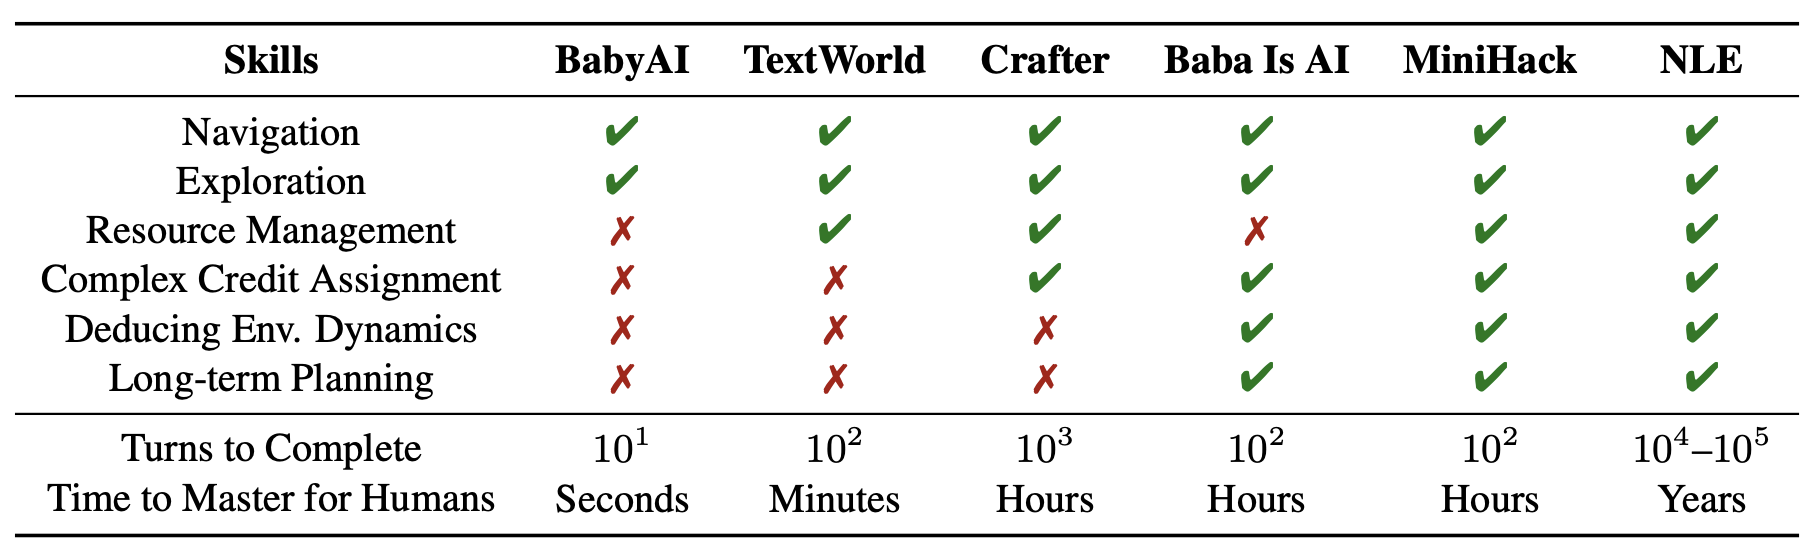
\includegraphics[width=0.98\linewidth]{figures/balrog}
    \caption{BALROG 中的游戏列表 \citep{paglieri2024balrog}}
    \label{fig:balrog}
\end{figure}

BALROG 旨在用推理问题挑战上下文式智能体。
它用谜题式游戏来评测大语言模型与视觉语言模型的推理能力。图~\ref{fig:balrog} 列出了这些游戏。游戏由易到难为：BabyAI、Crafter、TextWorld、BabaIsAI、MiniHack、NetHack。这些游戏带来了多种挑战：有些基于文本，有些带视觉成分，全都包含对模型的推理挑战。其中一些游戏被视为高难度。例如，并不指望你的模型或你的智能体——或者你自己——能在 NetHack 上取得高分。（如果你在没看过攻略的情况下真做到了，也许可以考虑为某个顶尖人工智能会议写篇论文。）

\begin{comment}
BALROG is designed originally for in-context learning, where the agent is simply a prompt improver (such as Tree of Thoughts or ReAct). 
Only inference is necessary. However, some of the BALROG games are quite challenging. Nothing prevents us from going to the next level and to try metalearning, or finetuning, such as GRPO, RLVR, or ReFT. These advanced methods are for later, however, we will start with regular in-context learning.




\paragraph{Multi-step Reasoning}
In agentic LLM, we want our agents to be able to communicate in natural  language, but they should also be able to make intelligent decisions, to reason and to look ahead about the consequences of their actions. Reasoning benchmarks test these abilities. Many games make excellent benchmarks to test if an agent can do multi-step reasoning well. 

The games in BALROG are quite diverse: some are easy, some are hard. They allow us to test if chain of thought prompts are powerful enough to solve easy planning problems, and hard planning problems.

\paragraph{Self Reflection}
As we have seen in the previous chapters, chain of thought is sometimes not strong enough, and we want our agent to learn from its mistakes, to be able to self-reflect, to see if its reasoning should be adapted.

This brings us to metalearning, the problem of learning to solve a set of {\em tasks}, instead of just a set of examples (a single task).

%First of all we can see self improvement of the policy of actions, a single level of learning. You can also go a level higher, to metalearning, to try to improve the learning algorithm, as we saw in the last chapter. 

Before we jump into metalearning right away, we should first get a single level baselearner to work well, bug free, achieving stable learning, giving results that fit our intuition. 
Only if we have a stable baselearner whose behavior you understand, does it make sense to try to build a second level of learning on top of the baselearner. %The proverb about running and walking applies.
\end{comment}

\subsection{谜题与游戏}
BALROG 由图~\ref{fig:balrog} 所示的六种谜题与游戏构成。这些游戏从简单的网格世界谜题，到基于文本的高难度地牢与龙类策略游戏，后者具有长信用分配回合和平坦的奖励地形。

BALROG 的作者提供了一套代码库，可用来实验各种智能体、设计你自己的智能体、观察它们在基准上的表现。要在 BALROG 的基准上表现良好，智能体必须擅长推理与规划，而且很可能还要擅长适应和反思自身行为。


%Well suited for reasoning, testing planning capabilities of LLMs.

%* describe balrog: benchmark suite, puzzles and games, planning challenge


BabyAI 是一个简单的网格世界游戏，智能体必须完成一项导航任务。一个简单的强化学习式算法就能轻松解决这个游戏。任务用自然语言给出，例如：{\em 走到蓝球处，然后捡起灰色钥匙}。当然，对智能体式大语言模型而言，挑战在于完成其中的规划部分。可以预期大语言模型能在这个简单游戏上表现良好（见 BALROG 论文）。

另一方面，NetHack 是一款极具挑战性的游戏，对人类玩家也是如此。NetHack 是一款基于文本的、类似地牢与龙的游戏。它既包含
长期战略规划——赢下一局可能涉及数十万步——也包含为击退成群怪物而进行的短期战术战斗。在 NetHack 中，信用分配是一大挑战，因为要弄清智能体过去的哪些动作最终促成了成功或失败：游戏某一区域的动作可能在远处引发意想不到的后果，这使强化学习智能体难以应对。众所周知，人类玩家若不借助攻略，往往要花数年才能
精通这款游戏。

\begin{comment}
    
\subsection{Knowing-Doing Gap}

As we discussed in Section~\ref{sec:knowing},  LLMs are often able to {\em answer} questions about the game mechanics and optimal strategies (the cheat guides were presumably part of the pretraining corpus), but they often
fail to be able to  apply this knowledge in practice.  This phenomenon has been called the {\em knowing-doing gap}. An LLM may be able to recite an algorithm to solve a problem, but it is not able to correctly execute this same algorithm.  The knowing-doing gap occurs in the harder puzzles, where the agent is not able to execute planning and reasoning to the required level of precision. It starts making errors. LLMs are good at associative lookups, not at precisely keeping track of changes to the values of variables. See also Section~\ref{sec:knowing}.


For you, in your experiments,  the challenge is to see if you can get your system to work well enough that you can run (moderately) difficult problems, so that the knowing-doing gap  occurs, and, then, of course, if you can find a way to make your agents  overcome the gap.

\end{comment}

\begin{figure}
    \centering
    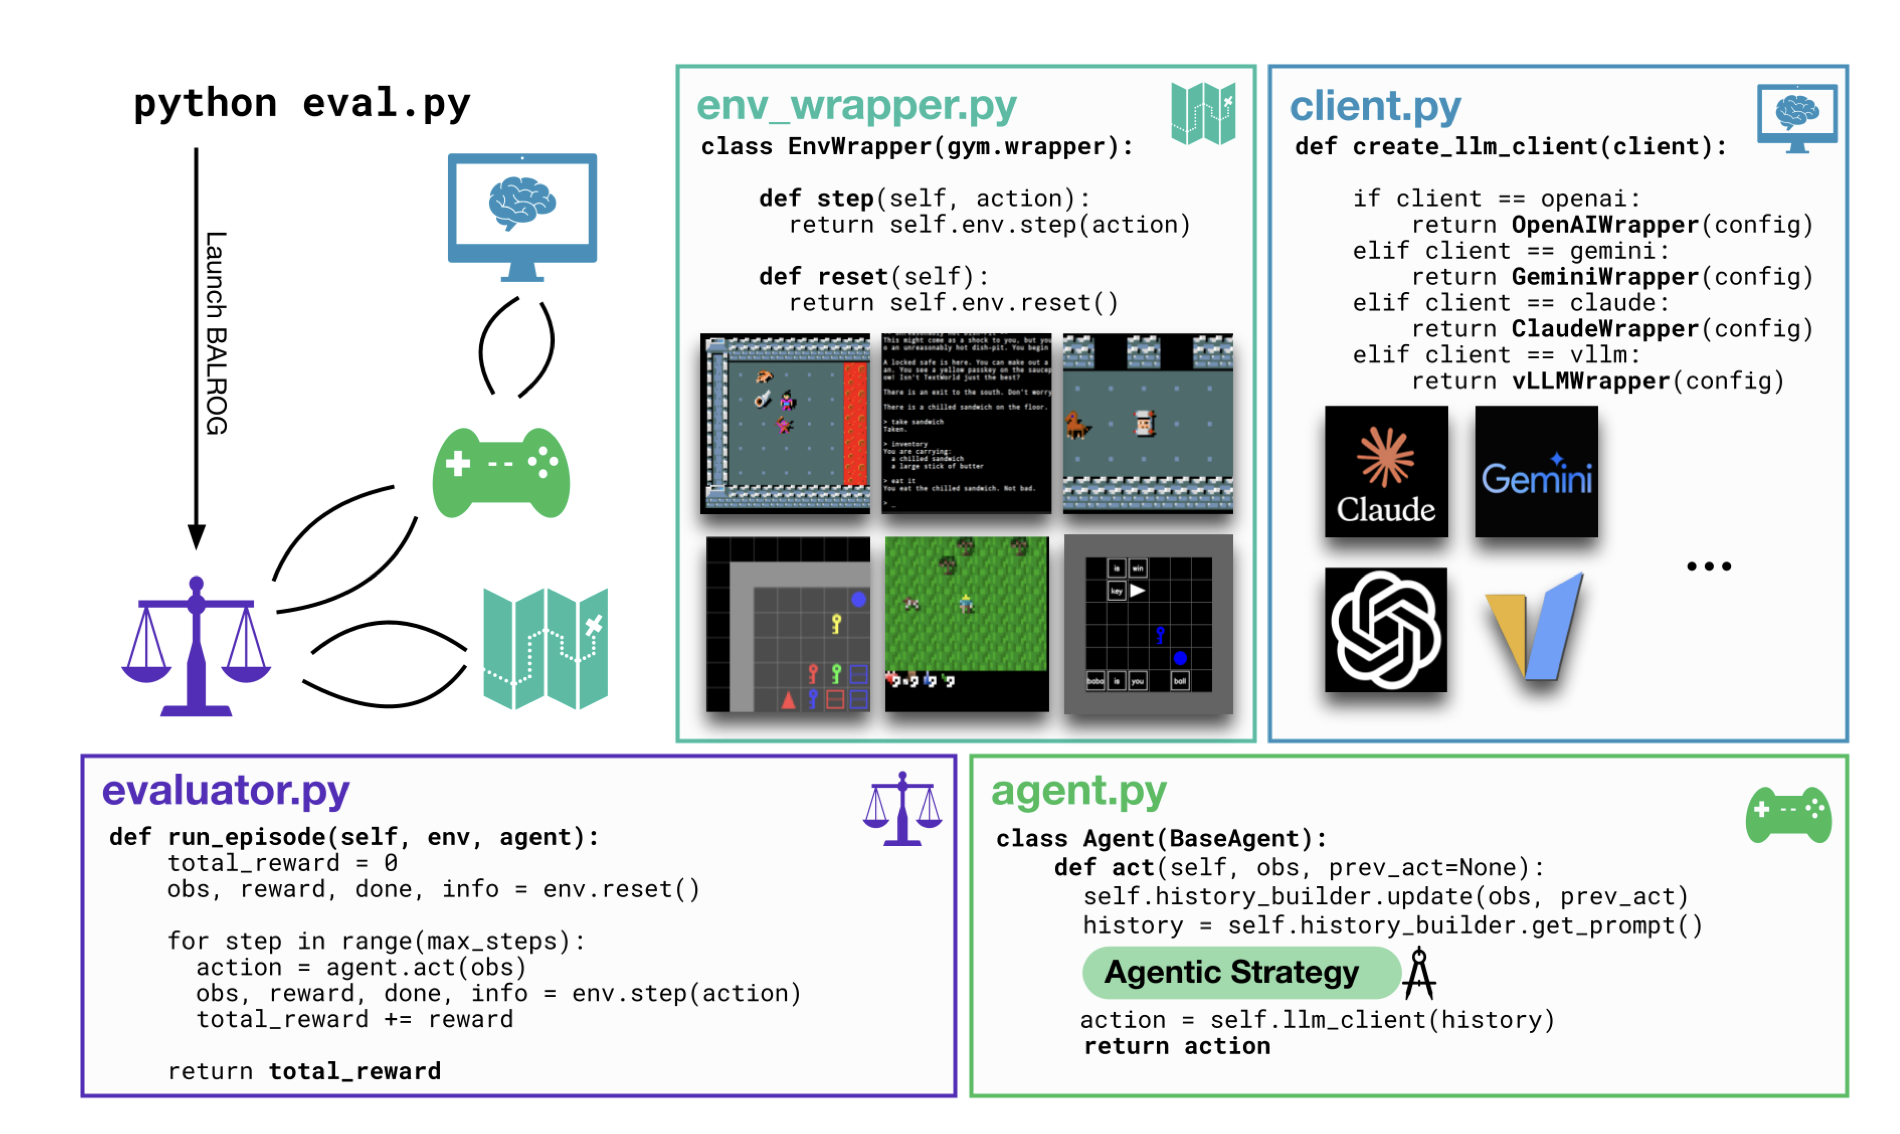
\includegraphics[width=\linewidth]{figures/balrogarch}
    \caption{BALROG 的架构 \citep{paglieri2024balrog}}
    \label{fig:balrogarch}
\end{figure}

\subsection{BALROG 架构}
现在来看 BALROG 框架的架构。图~\ref{fig:balrogarch} 展示了该架构，取自论文 \citep{paglieri2024balrog}。


%\subsection{Read Paper}
% - read paper to understand balrog goal \citep{paglieri2024balrog}.

请先熟悉 BALROG 系统。阅读论文 \citet{paglieri2024balrog}，可在 \url{https://arxiv.org/abs/2411.13543} 找到，或访问 BALROG 网站 \url{https://balrogai.com}。%(Many good papers in machine learning provide the code with their papers on Github, to ease reproducibility of their work.)


如果还没装，请用 \verb|git clone| 命令在你的系统上安装 BALROG。
访问 \url{https://balrogai.com}，或直接访问 GitHub 仓库 \url{https://github.com/balrog-ai/BALROG}。把该仓库安装到你的本地计算机上。

决定你要使用哪个大语言模型。请注意，典型的 BALROG 智能体在每一步都会进行大量大语言模型调用。如果你想在本地运行大语言模型，就安装它，或从 Huggingface 使用它。如果你想使用（商业）云端大语言模型，就申请一个 API 密钥并把该密钥配置到你的环境中。如果提供学生免费额度，你可以考虑申请。使用前沿大语言模型可能很昂贵，但通常更旧、更小的模型——其中一些仍相当有能力——要便宜得多。

GitHub 仓库上的 BALROG readme 包含如何安装该系统、以及如何为你喜欢的大语言模型配置 API 密钥的信息，见代码清单~\ref{lst:key}。（在某个练习中我们会使用多个大语言模型来比较它们的表现。眼下我们只是想让系统跑起来，用哪个都行。）
\begin{listing}
    \begin{minted}[
frame=lines,
framesep=2mm,
baselinestretch=1.0,
fontsize=\footnotesize,
linenos
]{bash}
        export OPENAI_API_KEY=<KEY>
        export ANTHROPIC_API_KEY=<KEY>
        export GEMINI_API_KEY=<KEY>
    \end{minted}
    \caption{配置 API 密钥}\label{lst:key}
\end{listing}

\subsection{智能体}
请阅读 BALROG 中的智能体教程：\url{https://github.com/balrog-ai/BALROG/blob/main/docs/agents.md}。在 BALROG 中，智能体是一小段 Python 代码，它用一个提示词调用大语言模型，以获得如何确定下一步的答案。智能体代码负责接收模型给出的回答（观测），并负责选择下一个动作。大语言模型被用来执行各种提示词。

BALROG 遵循图~\ref{fig:rlD} 中的交互范式 D，其中提示词由交互历史构建而成。

\subsubsection{提示词构建器}
智能体基于先前的动作、基于先前交互的观测/动作对来构建提示词。
因此，用强化学习的术语来说，智能体履行策略的职能：根据到来的观测选择要执行的下一个动作。

请到 \verb|prompt_builder| 目录，修改提示词由动作历史构建的方式。

\subsubsection{智能体}
智能体负责记忆功能：管理
观测/动作历史。
智能体必须记录过去的观测与动作，以支持上下文感知的决策，而这必须由我们在大语言模型之外实现。

BALROG 中的智能体代码会查询大语言模型：智能体把观测发给大语言模型，接收回答，并用这些回答决定在游戏中采取什么动作。

BALROG 自带若干预写的智能体，你应研究它们来设计自己的智能体。该仓库有一个朴素智能体和一个思维链智能体。此外还提供了更健壮的版本，用于处理大语言模型的回答。

当你构建自己的智能体时，你很可能会在自定义智能体基础上进行。
BALROG 智能体教程提供了一个简单规划智能体的例子。


\section{实现步骤}
下面提供一些练习，帮助你探索如何构建自己的智能体。
\subsection{复现论文}
%- task 1: implement standard task, reproduce.

我们先尝试复现 BALROG 论文中的结果。
请查看 GitHub 上的 BALROG 代码 \url{https://github.com/balrog-ai/BALROG}。阅读评测指南、智能体开发教程，以及如何运行少样本学习实验（上下文学习）的说明。
在你的计算机上安装相关工具和正确的 Python 版本（并把它加入 PATH）。在命令提示符下启动 Python 解释器来检查版本：\verb|$ python|。

首先，运行标准评测，以确认安装无误，见代码清单~\ref{lst:eval}。
\begin{listing}
    \begin{minted}[
frame=lines,
framesep=2mm,
baselinestretch=1.0,
fontsize=\footnotesize,
linenos
]{bash}
 python eval.py \
  agent.type=naive \
  agent.max_image_history=0 \
  agent.max_text_history=16 \
  eval.num_workers=16 \
  client.client_name=openai \
  client.model_id=gpt-4o-mini-2024-07-18       
    \end{minted}
    \caption{运行标准评测}\label{lst:eval}
\end{listing}




\subsection{不同的语言模型}
%- task 2: try different models, run local/api, use wandb.ai, setup extensive experiment chain

为了感受标准智能体在不同基准上配合不同大语言模型的表现，运行几个不同的大语言模型会很有用。%When you are using the API version, this requires acquiring different API keys, which may cost you money, or finding out which free tiers for students are possible. 
建议同时运行闭源和开源大语言模型，看看它们的表现。尤其是来自 OpenAI、Claude、DeepSeek、OLMo 和 Qwen 的开源版本可能表现良好。

运行这些模型很重要，能让你对大语言模型各自的相对优势有更多洞见。

\subsection{不同的谜题}
%- task 3: try different puzzle problems, understand the problems
接下来，为了更好理解该基准，在不同谜题中运行大语言模型智能体之后，你应仔细查看提示词与大语言模型的回答。看看能否发现大语言模型智能体在哪里失败、智能体的弱点在哪里。通过仔细检查单个动作、并更深入理解谜题，你也许能想到改进智能体的办法。

\subsection{计算成本}
BALROG 智能体在智能体每走一步时都会调用一次大语言模型，提示词往往很长。在这些谜题与游戏中会产生许多这样的步骤。在完整基准上、对不同的随机种子运行不同的大语言模型，很容易消耗大量词元。

在你的实验中，先试一个又小又便宜的大语言模型，例如 Qwen-3B。从最简单的基准（BabyAI 和 Crafter）开始。如果你想扩展，请便，但要注意计算成本。你想要洞见，但也希望实验能在合理的时间内以合理的成本完成。

\subsection{实现自己的推理智能体}
%- task 4: implement own agent, baselearner. 
现在该实现你自己的学习智能体了。
到 balrog 的 agents 目录，编辑 \verb|custom.py| 文件。
代码清单~\ref{lst:agent} 复现了 BALROG readme 中 Custom Agent 的代码。该代码可用代码清单~\ref{lst:agent-run} 中的命令运行（指定自定义智能体，并用较少的工作进程温和运行）。当然，你可以在命令中指定自己选择的大语言模型。

从提供的代码开始，运行它，看看它如何工作。然后，你可以尝试做些小改进。试着修改给大语言模型的提示词，以及修改 Python 代码处理智能体中学习的方式——可以在历史提示词构建器里、在计划里，或在学习算法里。

\begin{listing}
\begin{minted}[
frame=lines,
framesep=2mm,
baselinestretch=1.0,
fontsize=\footnotesize,
linenos
]{python}
from balrog.agents.base import BaseAgent
import re


class CustomAgent(BaseAgent):
    def __init__(self, client_factory, prompt_builder):
        super().__init__(client_factory, prompt_builder)
        self.client = client_factory()
        self.plan = None

    def act(self, obs, prev_action=None):
        if prev_action:
            self.prompt_builder.update_action(prev_action)
        self.prompt_builder.update_observation(obs)

        plan_text = f"Current Plan:\n{self.plan}\n" if self.plan else "You have no plan yet.\n"

        planning_instructions = """
Review the current plan above if present. Decide whether to continue with it or make changes.
If you make changes, provide the updated plan. Then, provide the next action to take. 
You must output an action at every step.
Format your answer in the following way:
PLAN: <your updated plan if changed, or "No changes to the plan." if the current plan is good>
ACTION: <your next action>
        """.strip()

        messages = self.prompt_builder.get_prompt()
        if messages and messages[-1].role == "user":
            messages[-1].content += "\n\n" + plan_text + "\n" + planning_instructions

        response = self.client.generate(messages)

        # 从大语言模型的回答中提取计划与动作
        plan, action = self._extract_plan_and_action(response.completion)

        # 若计划有变化，则更新内部计划
        if plan != "No changes to the plan.":
            self.plan = plan

        # 把计划存入 response.reasoning 字段，把动作存入 response.completion
        response = response._replace(reasoning=plan, completion=action)
        return response

    def _extract_plan_and_action(self, response_text):
        plan_match = re.search(r"PLAN:\s*(.*?)(?=\nACTION:|\Z)", response_text, re.IGNORECASE | re.DOTALL)
        action_match = re.search(r"ACTION:\s*(.*)", response_text, re.IGNORECASE | re.DOTALL)

        plan = plan_match.group(1).strip() if plan_match else "No changes to the plan."
        action = action_match.group(1).strip() if action_match else None

        return plan, action
\end{minted}
    \caption{BALROG 中的智能体代码}\label{lst:agent}
\end{listing}

\begin{listing}
    \begin{minted}[
frame=lines,
framesep=2mm,
baselinestretch=1.0,
fontsize=\footnotesize,
linenos
]{bash}
python eval.py \
  agent.type=custom \
  agent.max_image_history=0 \
  agent.max_history=16 \
  eval.num_workers=64 \
  client.client_name=openai \
  client.model_id=gpt-4o-mini-2024-07-18        
    \end{minted}
    \caption{运行智能体评测}\label{lst:agent-run}
\end{listing}

\section{评测}
BALROG 会把你的智能体表现报告为一个推进百分比。记录你尝试的每种基准和每种智能体类型的推进数值。要有条理地做这件事：你可以写一个 Python 或 shell 脚本来自动化运行实验和记录结果，或许还可以把推进情况画成图表。可以考虑使用 wandb.ai。

哪些智能体类型表现好，在哪个基准上表现好？做一张矩阵表，记录你尝试的智能体类型与基准类型各自的推进情况。

注意，大语言模型实验本质上是非确定性的：同一提示词两次运行可能给出不同结果。因此，每个实验要做多次运行。如果连续五次得到完全相同的结果，你或许可以开始相信这些结果。如果结果差异很大，你或许该去调查一下。原因纯粹是统计性的吗？调低温度能解决问题，还是有别的问题？

不要盲目相信所报告的推进数值。既然你是在计算机上运行代码，就可能存在缺陷或其他问题。BALROG 系统便于深入探究每次运行。它会记录 csv 文件，你可以用电子表格查看。看看其中一些运行记录，判断你看到的是否合理，还是智能体表现出退化行为。如果出现退化，试着找出原因。是你做错了什么吗？基准与智能体行为之间是否存在意想不到的相互干扰？
奖励地形是否过于平坦，以致智能体没有可追寻的信号，只是毫无意义地原地打转、随机动作？对此你能做些什么吗？

请注意，大语言模型领域、尤其是智能体式大语言模型领域是新的，我们的认识和软件框架尚未稳定。出现一些意想不到的结果是可以预期的，也会有一些挑战乃至挫折。

有条理的实验与结果记录方式是你的朋友。规划与组织能让实际智能体式大语言模型实验的运行、评测与改进成为一件愉快的事。

\section{自反思}
当你能够复现基准结果、并对智能体做了一些实验之后，你也许想尝试更大的挑战。本节我们将尝试把 BALROG 智能体扩展到自反思，其中大语言模型被用于不同角色，如评测和动作选择。自反思如同任何追逐一个自身也在被优化的目标的自适应系统一样，容易不稳定和振荡。因此，在我们尝试自反思想法之前，上一小节的基学习器系统必须能正常工作，并以稳定、可预测的方式收敛。
请回到那一小节，确保一切如你所愿地工作。

近来有许多试图改进大语言模型智能体的工作。我们提两个：ReAct \citep{yao2022react} 与 reflexion \citep{shinn2024reflexion}。ReAct 主要聚焦提示词，而 reflexion 引入了新的智能体算法，包括短期与长期记忆。

\begin{figure}
        \centering
    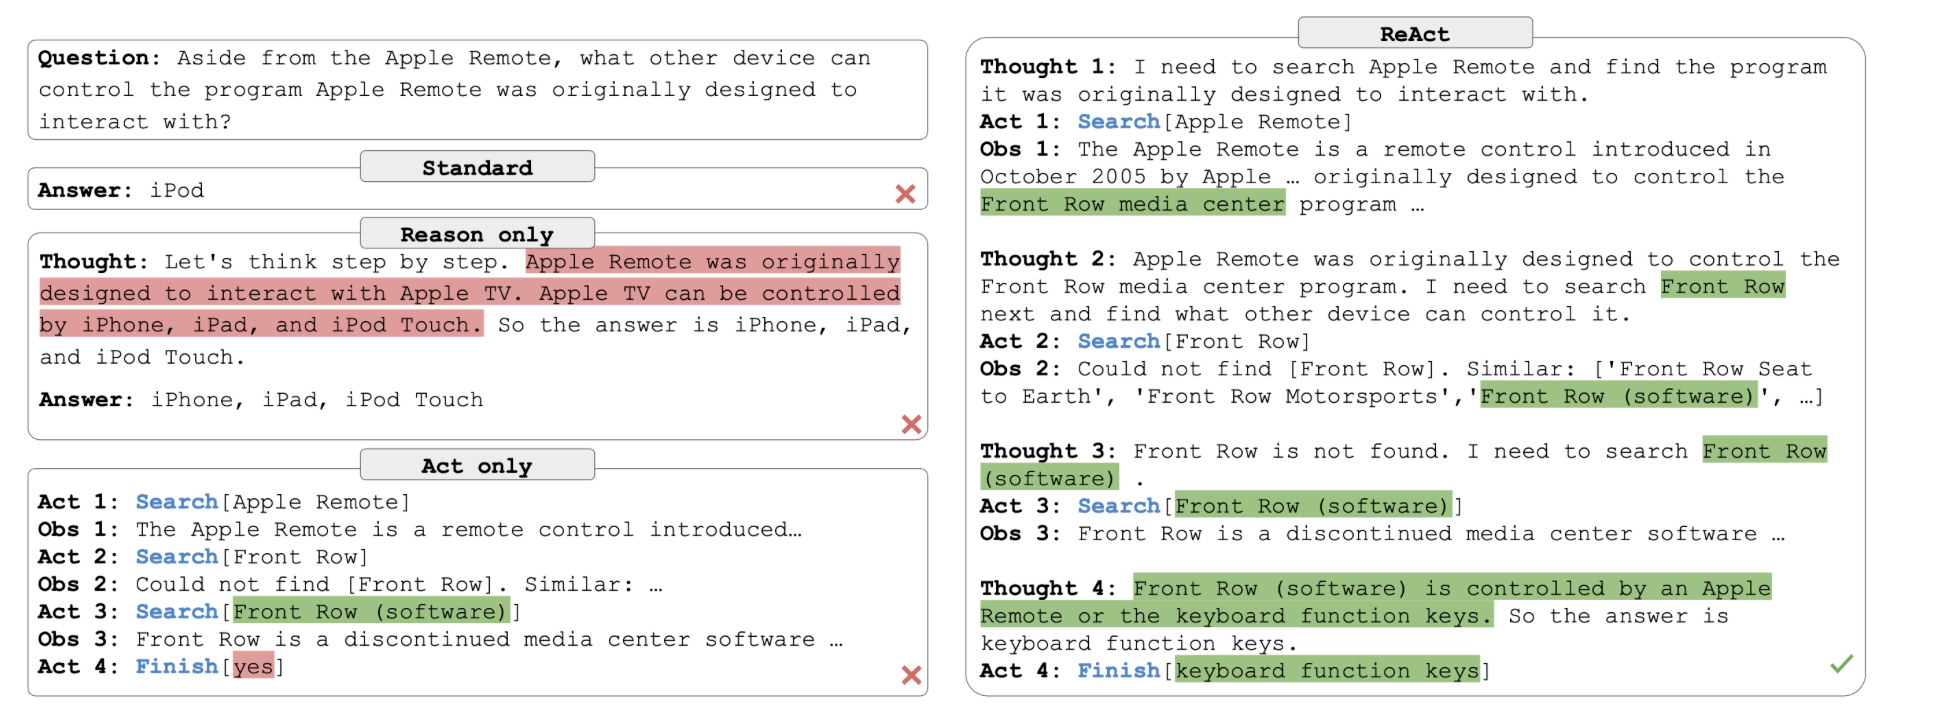
\includegraphics[width=0.95\linewidth]{figures/react}
    \caption{ReAct 执行搜索的示例 \citep{yao2022react}}
    \label{fig:react}
\end{figure}

\paragraph{ReAct}
ReAct 用提示词与世界交互。ReAct 提倡使用工具来查询信息，见图~\ref{fig:react}。ReAct 的原始网站是 \url{https://react-lm.github.io}，代码仓库在这里：\url{https://github.com/ysymyth/ReAct}。ReAct 提示也已在 LangChain\footnote{见 \url{https://docs.langchain.com/oss/python/langchain/overview}} 和 BeeAI\footnote{见 \url{https://github.com/i-am-bee/beeai-framework/blob/main/python/examples/agents/react.py}} 框架中实现。

看看这些框架，以理解 ReAct 所引入的基于提示词的智能体交互范式。然后，在 BALROG 中实现基于提示词的交互。它改善表现了吗？对哪些游戏，查询外部信息有帮助？对哪些游戏没有？

%- task 5: try self reflection. 

\paragraph{Reflexion}
ReAct 是基于提示词的，允许交互式查询；而 reflexion 办法引入了用 Python 编码的智能体，允许更精细的智能体行为。
Reflexion 在不同上下文、用不同提示词使用同一个大语言模型。
它基于这样一个假设：批评现有提示词哪里不对，比想出一个能用的提示词更容易。

Reflexion 是一种流行的自反思架构 \citep{shinn2024reflexion}。reflexion 的主网页是 \url{https://github.com/noahshinn/reflexion}。一篇介绍 reflexion 主要思想的博文在这里：\url{https://nanothoughts.substack.com/p/reflecting-on-reflexion}。

\begin{figure}
    \centering
    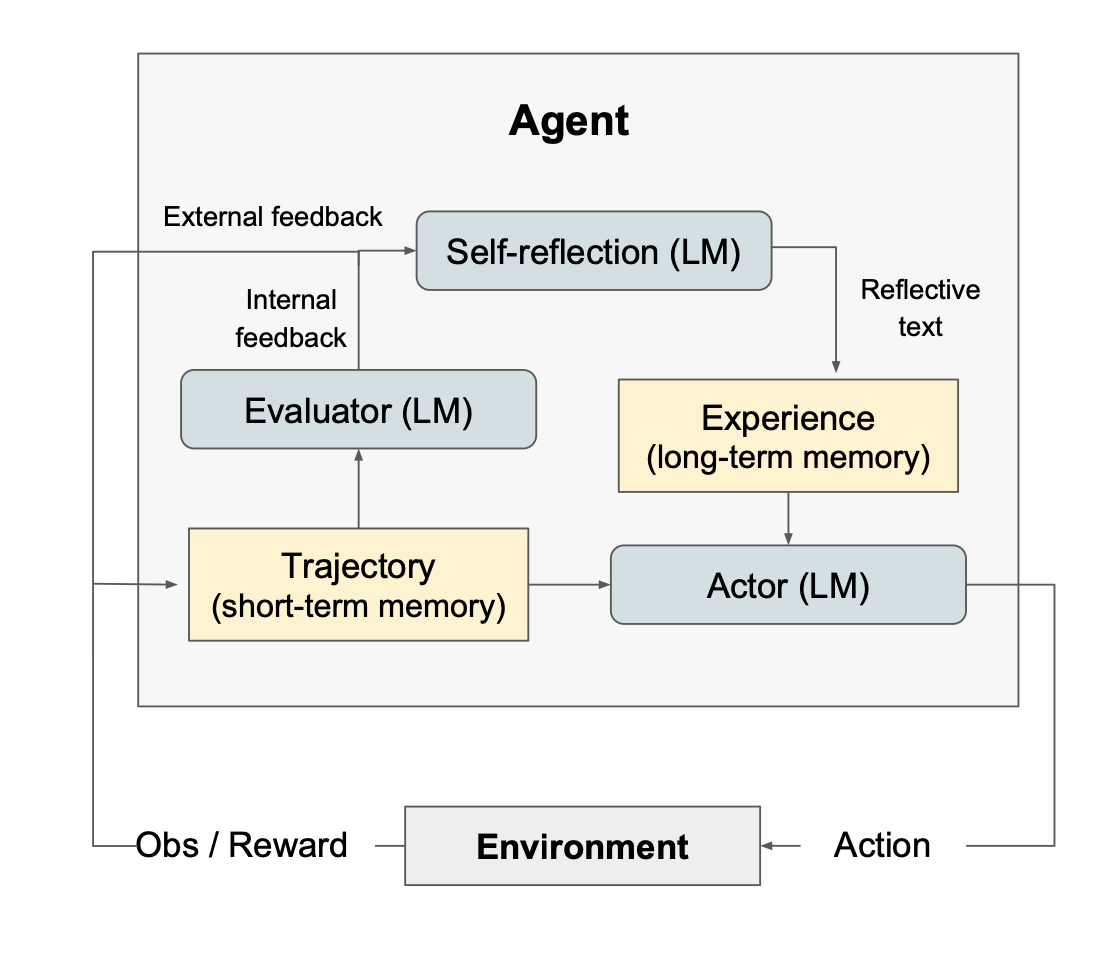
\includegraphics[width=0.5\linewidth]{figures/reflexion3.png}
    \caption{Reflexion 架构 \citep{shinn2024reflexion}}
    \label{fig:reflexion-alg}
\end{figure}


\begin{figure}
    \centering
    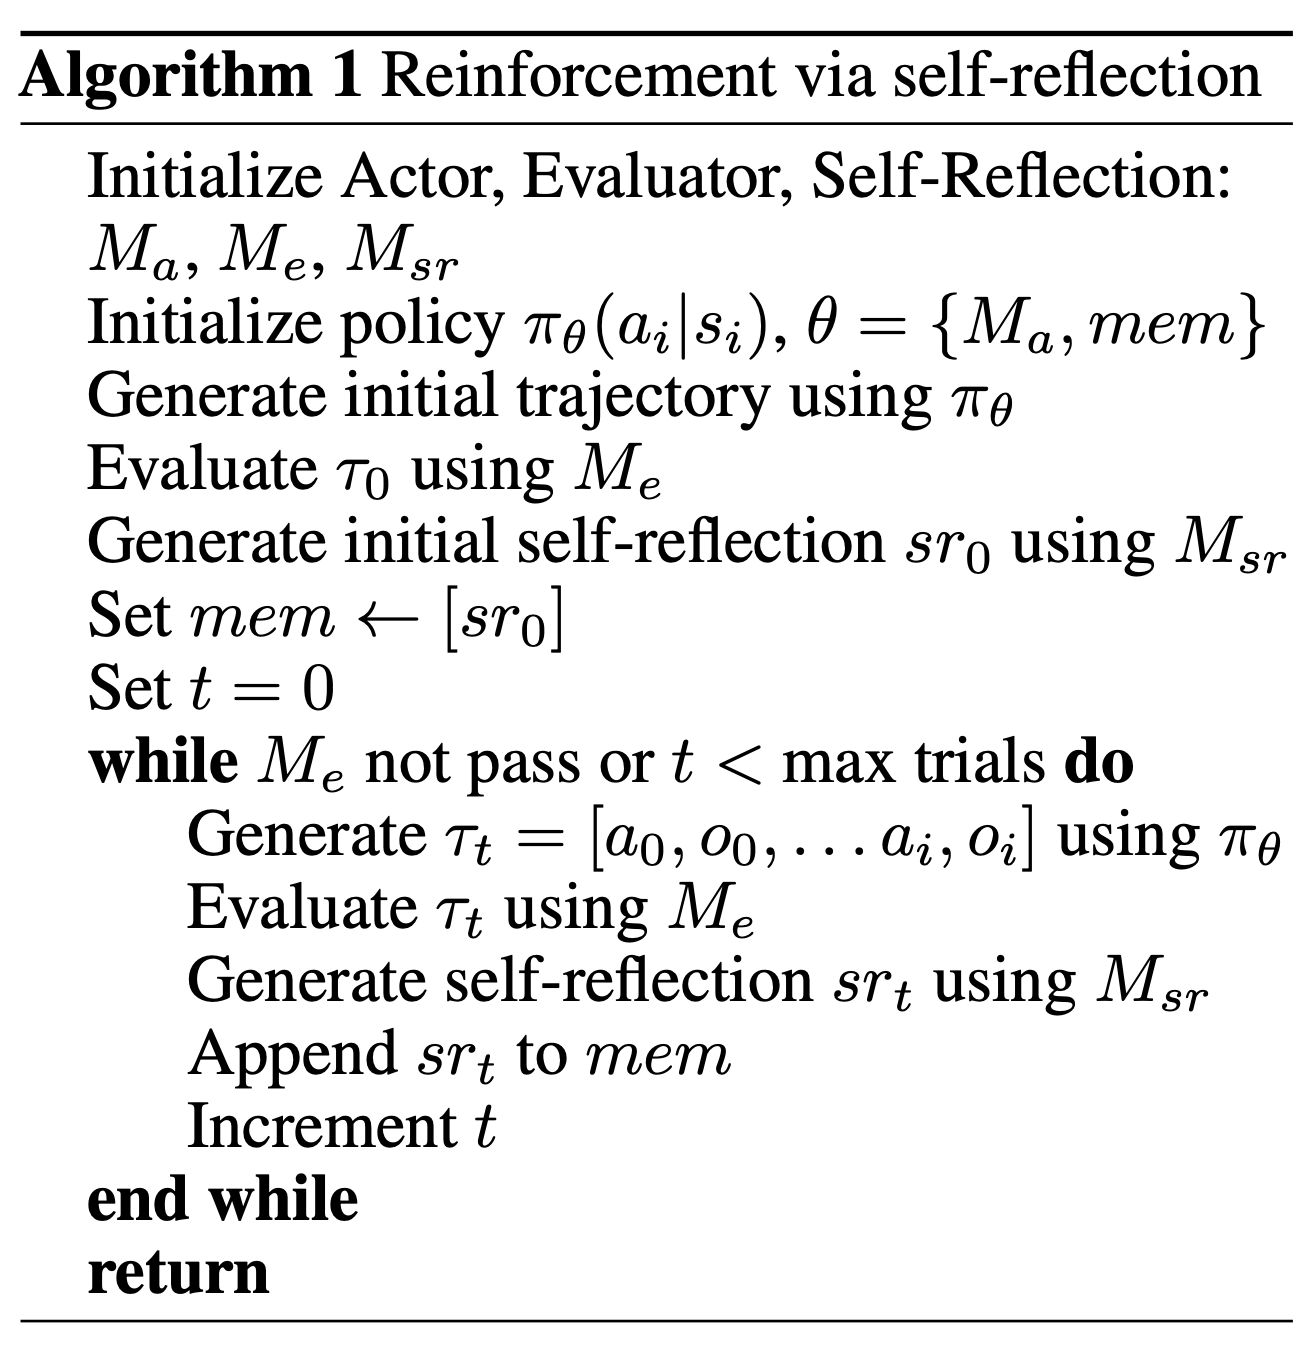
\includegraphics[width=0.5\linewidth]{figures/reflexion-code.png}
    \caption{Reflexion 算法 \citep{shinn2024reflexion}}
    \label{fig:reflexion-code}
\end{figure}

图~\ref{fig:reflexion-alg} 展示了 reflexion 的一般概念、不同的提示词以及不同类型的记忆。图~\ref{fig:reflexion-code} 展示了 reflexion 的代码，其中第 3、5、6 行（$M_a$、$M_e$、$M_{sr}$）与第 9、11、12 行有对大语言模型的不同调用。注意该代码是伪代码，关于记忆管理、提示词管理和收敛判据的重要细节都留空。
详情请查看 GitHub 上的仓库。

Reflexion 用不同提示词调用同一个大语言模型，这可能导致学习不稳定和循环。此外，记忆管理相对简单，存在上下文溢出的可能。一个想法是用 Python 手工实现分块或其他记忆压缩方法，或借助大语言模型来实现。

先玩一玩 reflexion 仓库，试着让它在 reflexion 的应用上跑起来，如 AlfWorld 和 HotpotQA。

\paragraph{扩展}
现在，试着在 BALROG 中实现一个 reflexion 智能体，在 BALROG 基准上运行。
你遇到了什么问题？reflexion 相比标准 BALROG 智能体改善表现了吗？

接下来，进一步扩展这个问题。你可以尝试在文献中寻找其他反思方法，或尝试自创新的反思方法。你可以尝试不同的应用类型，看看你的办法表现如何。当然，你也可以尝试其他大语言模型。

\section{结语}
本章讨论了一个实际案例研究，看看大语言模型如何执行自反思。我们使用了 BALROG，一套流行的推理任务基准。BALROG 由从易到难的混合游戏构成，其中一些连大语言模型都难以玩好。
BALROG 套件以开放风格设计。我们可以编写自己的智能体代码，然后可在 BALROG 游戏上运行。

这是一个重要的实际案例研究。
你已探索了为上下文推理编写自己的智能体代码。你还超越了基学习，实现了自反思。你在不同大语言模型上和极具挑战性的基准上，探索了自反思的稳定性。

%In this chapter, you have gained experience with state of the art problems in the field.
%
%The field is young, and not all problems have been resolved. LLMs are powerful, but there are certainly problems that they cannot solve. Some of these problems are planning related, such as the problems in the BALROG suite. This is an active area of research, and new methods will be invented that will perform better on planning problems. Another challenging problem is the knowing-doing gap. This is also an active area of research.




\begin{comment}
    
Set API-key

Choose configuration parameter.

go to naive agent

\begin{enumerate}
    \item Read the BALROG paper to understand the point of the benchmark
\item First decide on running locally and setting up your infrastructure.
\item Second install BALROG.
\item Third try to run the example code, generate graphs, check them with the paper.
Run it for the simple benchmark, and for the harder ones, to get a feeling for the problem that BALROG agents are meant to address.
\item Write a simple custom agent. Perform experiments. Does it solve simple benchmarks? Harder ones?
\item Write a more elaborate agent, for example based in Tree of Throughts, or ReAct. See how it performs on easy and on hard benchmarks. Does it do self-reflection?
\item Write a metalearning approach. What does it mean to do metalearning in a gaming environment? What is the inner loop, what is the outer loop?
\item Can you think of even more elaborate self reflection approaches?
\end{enumerate}


\subsection{Agent Development}

Run the planning agent.

implement prompt improver.

Look at tutorial

Implement ReAct

\end{comment}


\bibliographystyle{plainnat}
\bibliography{agenticbook,refs,case,synthetic}
